\chapter{Algorithms and Data Structures for mtDNA Sequence Alignment}
\label{chapterAlignment}
\label{chap:alignment}
The algorithm of life is based on a set of building blocks, that are passed on to the next generation, based on the concept of enormous redundancy \cite{DO90}. Thereby the concept of evolution is to reuse and modify successful building blocks (i.e. sequences or structures). Genes present in fruit flies are highly similar to those in humans, features that are associated with mtDNA mutations in vertebrates are conserved in fruit flies with comparable somatic mtDNA mutation frequency (${\sim 10})^{-5}$) \cite{Itsara2014}. Obviously both species do differ significantly from each other. While redundancy and similarity play an important role, the differences and conservation between sequences (encoding complex structures and mechanisms) are essential. To make any statements about the differences, various different sequences need to be aligned. The alignment of sequences is thereby one of the most central problems in the field of computational biology. Performing an alignment allows to detect and compare mutations, so called single nucleotide variants or polymorphisms, as well as short insertions and deletions (indels), being essential for DNA, RNA or amino acid sequence interpretation \cite{Gusfield1997}. According to Gusfield, high sequence similarity implies functional or structural similarity.  
\iffalse
Besides Next-Generation Sequencing devices distributing rapidly in the labs around the globe, Sanger sequencing is still used in Labs for DNA sequencing\footnote{https://www.lifetechnologies.com/at/en/home/life-science/sequencing/sanger-sequencing.html}. It is the workhorse that made it possible to determine the complete sequence of roughly 3.2 billion bases of the human genome in a time span of 13 years. Thereby it is very accurate, with fewer than one error per 10,000 bases\footnote{http://www.genome.gov/11006929}, corresponding a Phred quality score of $\geq$ 40. Most NGS devices show an error per base rate of Phred quality score 30 or below, third generation devices like the Oxford Nanopore show sequencing errors with Phred quality scores ~10 \cite{Ip2015} (indicating 10 errors on 100 basepairs), however yielding long reads of several kilobases. 
\fi

As abstracted in the introduction (Chapter \ref{chapterIntro}), different methods do exist to read out DNA and RNA sequences. Thereby the data generated by the sequencing devices comes as sequences of the alphabet set \(\{A, C, G, T\}\) whereby some special characters are used such as \textit{:} or \textit{d} representing one deleted base, - representing deleted base of unknown length, \textit{N} for any base, \textit{R} for purine (A or G), \textit{Y} for pyrimidine (C or T) called heteroplasmic mutations. The base sequence is essential, but gains even more importance if it can be compared to other sequences. So, having obtained the consensus sequence with one of the different ways of date generation in the lab, the issue now is to compare those sequences. This is of great importance in the field of phylogeny and evolution, but is also applied in gene discovery and detection of function of proteins to already known domains. This Chapter therefore gives an overview on this central problem in bioinformatics: sequence alignment, by focusing on the short circular mitochondrial genome sequence. The problem of alignment here is that a software generates only one of many possible representations. Different interpretation of insertion, deletions or transition / transversion can results to different nomenclature, limiting the interpretation and in the worst case resulting in wrong statements about pathogenic mutations or the misidentification of criminals (like the misidentification of Jack the Ripper\footnote{\url{http://www.independent.co.uk/news/science/jack-the-ripper-id-hinges-on-a-decimal-point-as-scientists-flag-up-dna-error-in-book-that-claims-to-9804325.html}} where we raised concerns about the correctness of the data). To prevent such a misinterpretation the concept of a recommendation system, based on a larger reference panel is introduced, and implemented as part of the HaploGrep system. Prior to that, this chapter gives the background of the alignment problem, with solutions and validation of related methods.

\section{Background: Mind the gap}
The alignment of two sequences $S_1$ and $S_2$ $\in \{A,C,G,T,N\}*$ (where $N$ is a placeholder for $A, T, G,$ or $C$) is a computation problem with complexity $\mathcal{O}(n \times m)$, where n =length $S_1$ and m= length $S_1$. For pairwise comparison of mitochondrial genomes, this corresponds $\mathcal{O}({n}^{2})$. For aligning $S_1$ and $S_2$, $\binom{n+m}{m} \sim \frac{ {2}^{m  + n}}{\sqrt[]{\pi m}}$\footnote{\url{http://www.cs.columbia.edu/4761/notes07/chapter2.1-Alignment.pdf}} different possible alignments can exist. However only a small subset of all possible alignments are biologically meaningful. To weight the different alignments, the simplest form would be to use the Hamming Distance (see \ref{hamming} and count the mismatches between two sequences D($S_1$,$S_2$). However the differences between two nucleotide sequences are not just single nucleotide variants, but can be present as insertions and deletions, rendering the Hamming Distance in this context merely useless. Also, the sequences can be of different length, being of requirement for the calculation of this distance. To cope with the gaps in form of insertions and deletions, the Levenshtein-distance, (often referred to as edit distance, shuffle-Hamming distance or Hamming+Gap metric) \cite{Deza2009} was introduced in 1965. It is based on a set of edit operations - copy or match (M), substitute or replace (R), insert (I) and delete (D). Thereby this operations build a string over the alphabet (M, R, I, D), describing the transcript from one sequence to the other (see Gusfield Chapter 11) \cite{Gusfield1997}, where the operations can have different weights ($w_M$=0, $w_I$=1, $w_D$=1, $w_M$=1). The following listing represents the transcript string between the sequences $S_1$ = ATCAGACGAG and $S_2$ ACAGGCGAT:
\begin{center}
\texttt{ATCAGACGA G} \\
\texttt{A CAGGCGATG} \\
\texttt{-----------} \\
\texttt{MIMMMRMMMDM} \\
\texttt{01000100010} \\
\end{center}
The edit distance is the minimum number of weights (i.e. edit operations, for all replace, insert and delete operations). This approach is part of inexact string matching class (see \ref{inexact}). Alternatively exact string matching approaches do exist, that are outlined in the subsequent section \ref{exact}. 

\subsection{Exact String Matching}
\label{exact}
The problem of exact string matching, is to find all occurrences of a string $P$ called \textit{pattern} and $T$ called the \textit{text}, by exactly finding the pattern $P$ as substring of $T$. While this might sound like an simple problem, the worst case running time for the naive method is $\mathcal{O}({n}\times{m})$ where $n$ denotes the length of $P$ and $m$ denotes the length of the text $T$.
\subsubsection{Naive Algorithm}
The naive algorithm takes the text $T$ and the patterns and $P$ as input by checking for each sequence of length $i = 1, 2, 3, \cdots m-n+ 1 $ if a substring in T can be found such that $t_i \cdots t_i+m = P$. This approach can be reduced to $\mathcal{O}({n}+{m})$
\subsubsection{Boyer-Moore Algorithm}
The Boyer-Moore Algorithm is an extension of the naive algorithm, based on 3 different rules, which improve the runtime significantly. 
\begin{itemize}
\item[1] \textbf{right to left scan in $P$}, which is not an optimization per se, but is used for the both rules, 2 and 3. 
\item[2] \textbf{bad character shift rule}: start with comparing pattern $P$ with text $T$ from left to right, while applying rule 1 for pairwise comparison of $P$ and $T$. Until a mismatch happens, compare $P_i$ with $T_{|P_i|}$, with i $\in (0,\cdots |P|)$ . If mismatch occurs, skip alignment until the next character in $P$ matches the mismatch on $T$ or skip the complete P and proceed on $T_{|P_i|}$. Figure \ref{fig:boyer2} represents the rules 1 (green arrow scanning right to left), and the 2 mismatches for the bad character shift rule.
\begin{figure}[!ht]

    \centering
    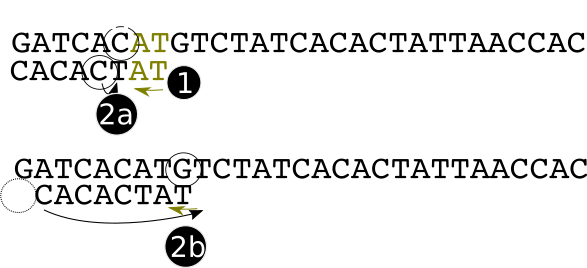
\includegraphics[width=0.6\textwidth]{images/boyer2.png}
    \caption[Boyer-Moore - example rule 1 and 2]{Boyer-Moore - example for rule 1 and 2. Pattern $P$ = \texttt{CACACTAT} is scanned from right to left. In 2a, a mismatch in the Text on position 3 happens. Subsequently $P$ is shifted for the next C, so that it matches with this position. Since in 2b no G can be found in the $P$, the complete string can be shifted behind this position on the text $T$.} 
\label{fig:boyer2}
\end{figure}

\item[3] \textbf{good suffix shift rule} This rule checks if a suffix from right appears subsequently after a mismatch. If the suffix $t$ can be found in $P$, alignments can be skipped and $P$ shifted - see Figure \ref{fig:boyer3} for an example.
\begin{figure}[!ht]

    \centering
    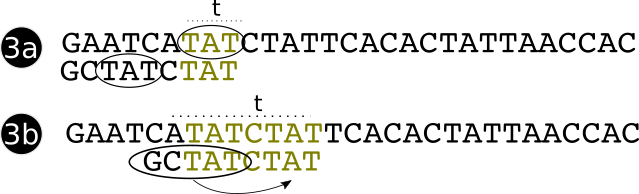
\includegraphics[width=0.65\textwidth]{images/boyer3.png}
    \caption[Boyer-Moore - example rule 3]{Boyer-Moore - example for rule 3. Subpattern $t$ = \texttt{TAT} is matches as suffix, and is 3 bases long, until a mismatch happens. Thereafter, good suffix is searched in $P$ with less search effort (3a). A suffix can also be repetitive, so that the the repetition skips alignments, by shifting to the first presence of In 2a, a mismatch in the Text on position 3 happens. Subsequently $P$ is shifted for the next C, so that it matches with this position. Since in 2b for the $P$ no G can be found, the complete string can be shifted behind this position on the text $T$.}
\label{fig:boyer3}
\end{figure}
\end{itemize}
The algorithm performs both rules and decides on the one that skips more alignment steps. A further step is the creation of a lookup table, where the number of skips are precalculated based on $P$. There do exist some more algorithms for exact string matching like the Knuth-Morris-Pratt algorithm or the 
\subsubsection{Offline Algorithm}
The previously described naive algorithm and its optimization the Boyer-More algorithm represent so called online algorithms (processing without an index). There is a second class of algorithms, based on the concept of preprocessing of the text $T$, by using an index. While this preprocessing step takes additional time and space, the overall runtime can be reduced significantly. Offline algorithms are also implemented in most modern web search engines.  The most notable offline algorithms are  k-mer or n-gram based search, suffix trees or metric trees. Since used in the subsequent sections, k-mer and suffix trees are shortly outlined within this paragraph.
\begin{itemize}
\item \textbf{k-mer} or \textbf{n-gram}: here the \textbf{k} or the \textbf{n} stand for the length of substrings of all possible occurrences in the text $T$. Figure k-mer gives an example with the text $T$ = \texttt{GAATGAATGC}, resulting in the sorted index. The lookup is often implemented as a HashMap, so that the generation of the index is $\mathcal{O}({n})$ and the query $\mathcal{O}({1})$
\begin{figure}[!ht]

    \centering
    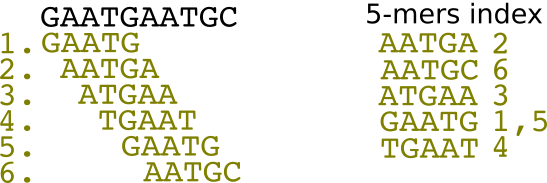
\includegraphics[width=0.65\textwidth]{images/k-mer.png}
    \caption[k-mer or n-gram]{k-mer or n-gram applied to the text  $T$ = \texttt{GAATGAATGC}. The k here is of length 5, so the index represents all possible 5-mers or 5-grams occurring in $T$. If for one entry, multiple positions in $T$ are be found (see \texttt{GAATG}, which starts on position 1 and 5), a Multimap can be used.}
    \label{fig:k-mer}
\end{figure}
\item \textbf{Suffix-Tree}
Suffix Trees are a very efficient data structures, to perform the exact string matching in linear time $\mathcal{O}({n})$. Thereby suffix trees are used to bridge the exact and inexact string matching problem \cite{Gusfield1997}. The preprocessing of the text $T$ with length $n$ requires  $\mathcal{O}({n})$, while the query for pattern $P$ of length $m$ requires $\mathcal{O}({m})$ to find the position of occurrence or find that the pattern is not contained. For constructing the tree, the symbol "\$" concatenated to the text. Now by iterating from the right of $T$, add nodes to the tree, for \$, C\$, GC\$, TGC\$ and so on. If a branch does start with the same characters, as the next suffix, add it under this branch and add the characters which differ to the neighboring branch, by adding the positions from $T$. Figure \ref{fig:k-mer} represents the finished suffix tree for  $T$ = \texttt{GAATGAATGC}. The implementation of a suffix tree was presented by Ukkonen in 1995 \cite{Ukkonen1995}, reducing the time complexity to $\mathcal{O}({n})$, otherwise requiring $\mathcal{O}({n^2})$ with a naive implementation.
\begin{figure}[!ht]

    \centering
    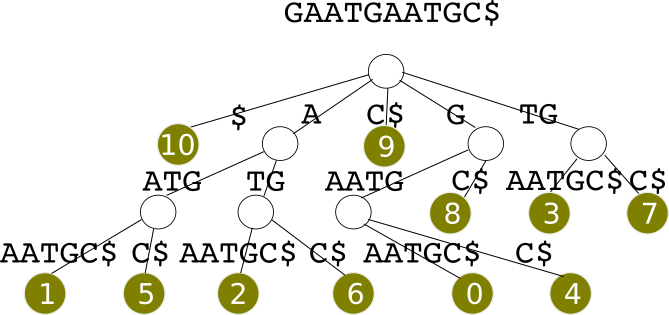
\includegraphics[width=0.8\textwidth]{images/suffixtree.png}
    \caption[Suffix Tree of String GAATGAATGC]{Suffix Tree of the text $T$ = \texttt{GAATGAATGC}. There do exist tools, that show the creation of such trees for educational purpose\footnote{\url{https://visualgo.net/suffixtree}}.}
    \label{fig:suffix}
\end{figure}
As can be seen in this example, the information can be redundant, so that improvements in the form of suffix array and FM-Index are used in computational biology. The suffix array is a ordered list of all suffixes, that can be directly be used for the FM-Index, based on the Burrows-Wheeler Transformation. This is used in most common mapping tools for DNA/RNA-read mapping, the most prominent being BWA \cite{Li2013a,Li2009} and Bowtie \cite{Langmead2009, Langmead2012}. While a suffix tree would need approx. 45GB of memory for the whole human genome DNA, the Suffix Array requires 12GB, and the FM-Index only about $\sim$ 1GB of memory \footnote{\url{https://www.coursera.org/learn/dna-sequencing/lecture/r8Xh3/lecture-genome-indexes-used-in-research}}. Figure \ref{fig:suffixarray} represents the steps that are applied to get the Burrows Wheeler Transformation from a suffix array.
\begin{figure}[!ht]

    \centering
    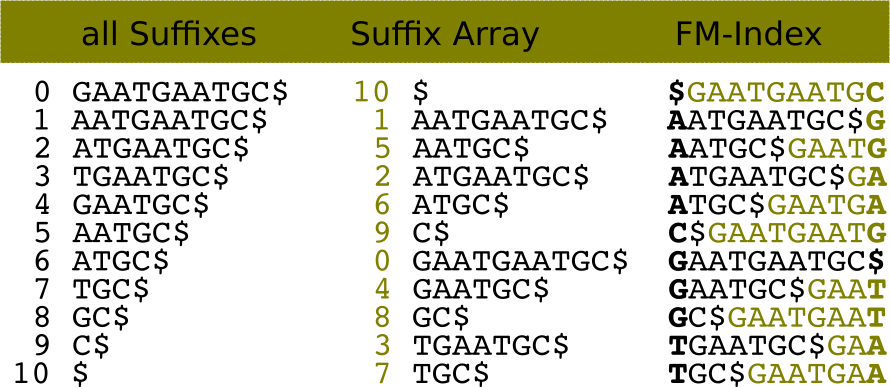
\includegraphics[width=1\textwidth]{images/suffix.png}
    \caption[Construction of suffix array]{Construction of suffix array, based on all suffixes, and ordered lexicographically ascending. The FM-Index extends the entries in the suffix array, by calculating the Burrows-Wheeler Transformation \texttt{CGGAAG\$TTAA} (last character (bold) of each row}.
    \label{fig:suffixarray}
\end{figure}
\end{itemize}
\subsection{Inexact String Matching}
DNA reads from modern devices, show much higher error rates, compared to Sanger based Sequencing. Third generation sequencing devices like MinION from Oxford NanoPore Technologies\footnote{\url{https://nanoporetech.com/products/minion}} showed a per base error with Phred-Score 7 (error rate $sim$ 15\%) with the initial chemistry R7. Even with the latest chemistry R9.4 used in the whole genome sequencing project of NA12878\footnote{\url{https://github.com/nanopore-wgs-consortium/NA12878}}, the error rate is about 10\% per base. Using exact string matching is not only limited by these errors, but also by the variation. The previously described Levenshtein distance or edit distance problem can be solved with  dynamic programming.      
\label{inexact}
\subsubsection{Dynamic Programming}
For solving the pairwise alignment problem, two different approaches are available, based on some similar underlying assumptions, solving however different problems. Both approaches rely on substitution scores, and are in  $\mathcal{O}({n m})$ for length $n$ and $m$ of two strings $S_1$ and $S_2$. The global or often referred to as Needlman-Wunsch alignment tries to align sequence pairs, so that all letters from both sequences are taken into consideration. The local alignment differs in this regard, by considering alignments, where the costs of a substring of either $S_1$ or $S_2$ can be improved compared to the global alignment. Both approaches are build by a matrix of size (n $\times $ m).
\subsubsection{Global Alignment}
The global alignment, addressed by Needleman-Wunsch \cite{Needleman1970}, contains all nucleotides from both sequences $S_1$ and $S_2$. A simple form of the substitution costs are 1 for match, 0 for mismatch and -1 for indels (gaps). Sequence $S_1$ and $S_2$ are used for column and rows in the matrix that will be used for dynamic programming. Figure \ref{fig:global} represents the two steps: filling in the score table, and walk back in the traceback table. For filling in the score table, the match/mismatch and gap scores are required. There are different predefined substitution matrices, like PAM250\footnote{\url{http://www.mbio.ncsu.edu/bioedit/tables/PAM250}} or BOSUM62\footnote{\url{https://www.ncbi.nlm.nih.gov/Class/FieldGuide/BLOSUM62.txt}}, widely used for amino acid changes. For the sake of simplicity, the score table is used 
as following:
\begin{figure}[H]

    \centering
    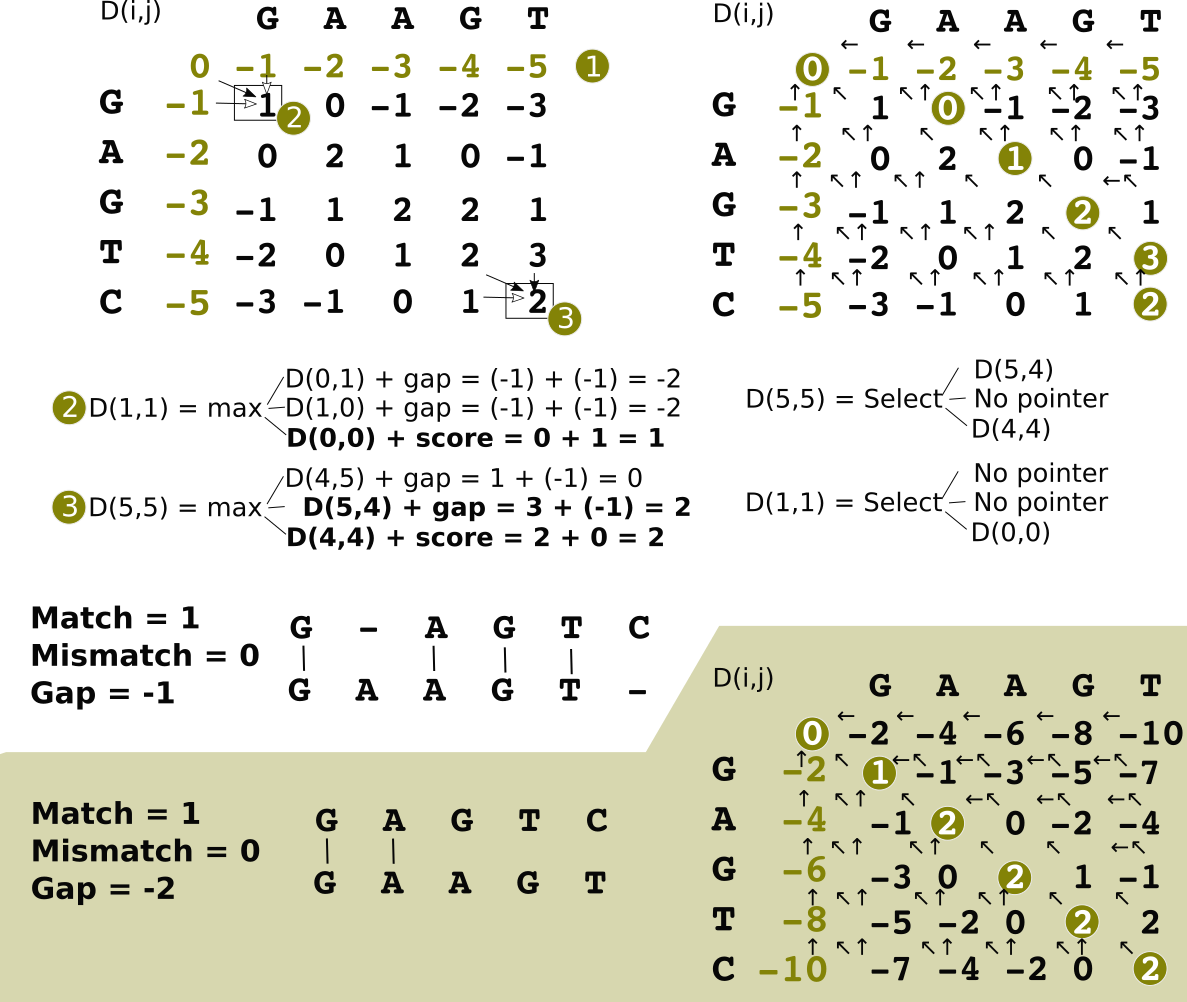
\includegraphics[width=1\textwidth]{images/globalAlign.png}
    \caption[Example of Global Alignment]{Example of Global Alignment, with 2 different gap scores (gap -1 and gap -2 (light-olive background)). The gap penalty and matching scores influence the alignment significantly, with two different results: 4 matches, 1 insertion and 1 deletion versus 2 matches and 3 mismatches.}
    \label{fig:global}
\end{figure}


\begin{table}[H]
\centering
\caption{Score Table, indicating the score for a match (1) and mismatch (0)}
\label{scoreTable}
\begin{tabular}{lllll}
  & \texttt{A} & \texttt{C} & \texttt{G} & \texttt{T} \\
 \texttt{A} & \cellcolor[HTML]{808000}1 &   &   &   \\
\texttt{C} & 0 & \cellcolor[HTML]{808000}1 &   &   \\
\texttt{G} & 0 & 0 & \cellcolor[HTML]{808000}1 &   \\
\texttt{T} & 0 & 0 & 0 & \cellcolor[HTML]{808000}1
\end{tabular}
\end{table}
In a first step, the gap penalty score is added in the first row, and first column, by summing up with the previous value (Figure 1, (1)). Subsequently the table is filled by recursively iterating over all entries in the matrix, and calculating the maximum value for the current cell $D_{i,j}$:
$ D_{i,j} = \max
  \begin{cases}
    D(i-1,j)+ \text{gap penalty}      \\
    D(i,j-1)+ \text{gap penalty} \\
    D(i-1,j-1)+ \text{matching score} \\
  \end{cases}
$


\subsubsection{Local Alignment} \label{localAl}
The Smith-Waterman algorithm \cite{Smith1981} as \textit{the} representation of a local alignment, is based on dynamic programming for finding substrings / regions of highly similar content. Since all possible alignments are considered, the optimal local alignment is guaranteed to be found. In the first step, the first column and first row are set to 0 instead to the gap-penalty score. Further a $0$ is added in the cases, so that negative entries are not possible. 
$ D_{i,j} = \max
  \begin{cases}
    D(i-1,j)+ \text{gap penalty}      \\
    D(i,j-1)+ \text{gap penalty} \\
    D(i-1,j-1)+ \text{matching score} \\
    0 \\
  \end{cases}
$\\
The filling of the scoring table is again a recursive step like in the global alignment. The traceback does not start in the cell D(n,m), but in the cell with the highest value. Figure \ref{fig:local} represents the same examples as for local alignment. Here the starting point for the traceback is however the highest entry in the scoring table. The end is reached by finding the cell with a value 0. This is very different from the global alignment, that always starts in cell $D(n,m)$ and ends in cell $D(0,0)$. Optimizations of this approach are presented by Gotoh \cite{Gotoh1982}.  
\begin{figure}[H]

    \centering
    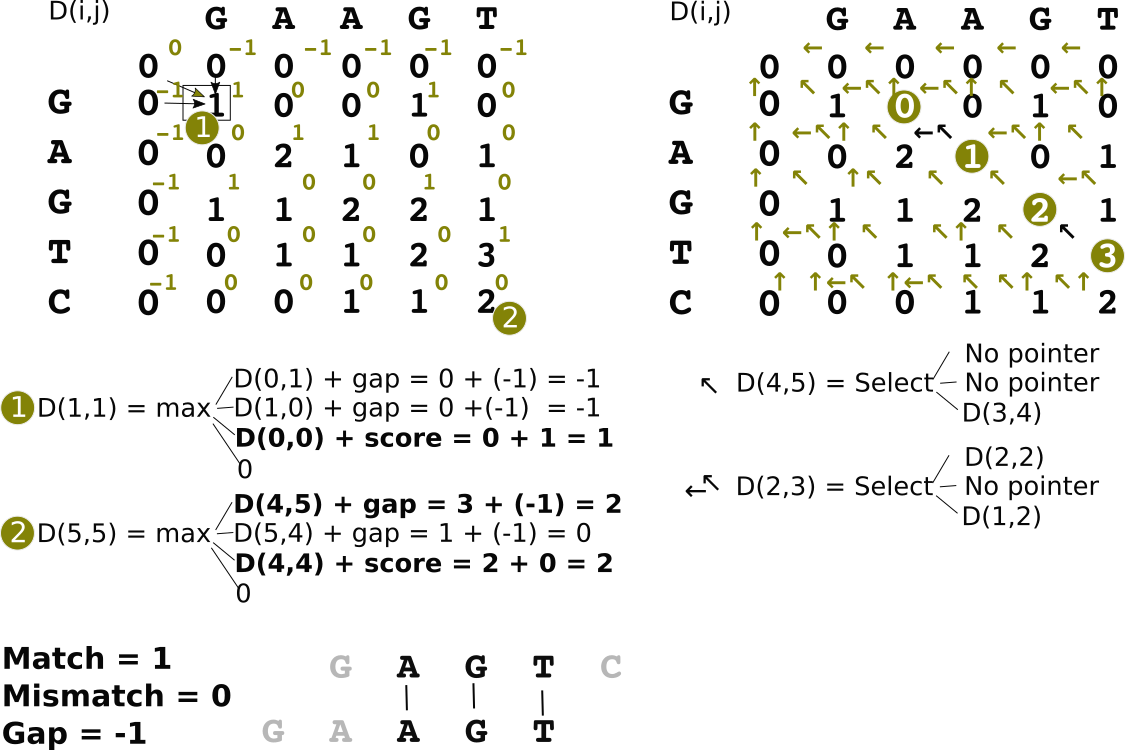
\includegraphics[width=1\textwidth]{images/localAlign.png}
    \caption[Example of local alignment]{Example of local alignment, with the Match/Mismatch/Gap scores as previously defined. As can be seen, only the part with the highest similarity \texttt{AGT} as substring of text $S_1$ and $S_2$ is the best result for the local alignment}
    \label{fig:local}
\end{figure}
%\subsection{Biological Networks}
\section{Aligning mtDNA sequences}
Although there exists plenty of alignment software performing pairwise alignment\footnote{see extensive list of pairwise sequence alignment tools here \url{https://omictools.com/pairwise-sequence-alignment-category}}, based on the previously described algorithms, the alignment for mitochondrial genomes comes with special requirements. Algorithms developed for the alignment of nuclear DNA often have issues with the correct nomenclature used for mitochondrial DNA. Also the circular structure of the mtDNA, where a start does not necessarily have to be at position 1 when linearized, needs further attention. 
\subsection{Related Work}
While there do exist approaches specifically for mtDNA, the available tools currently show slow run-times and are not suited for processing 1,000s of mtDNA sequences in feasible time. The next paragraphs present an overview of existent tools designed to align mtDNA sequences.
\begin{itemize}
\item \textit{MitoTool} accepts fasta files from either D-Loop (position 16024-574), the complete mtDNA sequences or to analyze mtDNA genome sequences lacking the D-loop region. However no information is provided about the algorithm used \cite{Fan2011,Fan2013}. The software is provided as web-server as well as a down-loadable version\footnote{\url{http://mitotool.org/software.html}}
\item \textit{MUMmer} is a suffix-tree based approach already described in the year 1999 \cite{Delcher1999} and updated to version 3.0 in 2004 \cite{Kurtz2004}. Currently version 4.0 is in preparation, updated to support multi-threading and genomes of any size\footnote{\url{http://mummer.sourceforge.net/} accessed March, 2017}. Although not explicitly designed for mtDNA, we will compare Mummer 3.0, since being integrated in HaploFind (see Chapter \ref{hg:related}) for the haplogroup assignment according the RSRS sequence.
\item \textit{mtDNAprofiler} \cite{Yang2013} is accessible via web\footnote{\url{http://mtprofiler.yonsei.ac.kr/}}. It implements two main rules, the first to use the least number of differences to the rCRS, and the second considering realignment of indels in the mtDNA like AC repeats or C-stretches in speficic regions. mtDNAprofiler can be used for up to 50 complete mtDNA sequences.
\item Further commercial alignment software exists, such as Sequencher\footnote{\url{http://www.genecodes.com/}}. It can be used for the alignment of any genomes or genes, but provides special rules in a forensic version for mtDNA\footnote{\url{http://www.genecodes.com/analyses/forensic-mitotyping}}, where the alignment can be modified. It requires an experienced user to correct the contigs consensus though. 
\item \textit{MitoTyper}: Several rules have been defined to overcome the special problems in the alignment of the mtDNA to the revised Cambridge Reference Sequence (rCRS)\cite{Andrews1999}. The first rules were designed by Wilson et al. \cite{Wilson2003} in the alignment an nomenclature protocol, the so called “Wilson rules”. These rules were generally accepted, but often led to ambiguous naming of the sequences. Budowle et al. \cite{Budowle2010} extended these rules for the human mitochondrial DNA control region. The reliability was shown on the Scientific Working Group of DNA Analysis Methods (SWGDAM) database\footnote{\url{https://www.swgdam.org/}}.Unfortunately we were not able to test either the commercial software nor to access the SWGDAM database. 
\item \textit{Phy-mer} \cite{Navarro-gomez2014} accepts full mtDNA sequences, and does not generate variant files, but rather performs a haplogroup comparison based on this k-mer, and alignment-free approach. This is done to avoid possible nomenclature errors, being very tricky. Phy-mer is available on GitHub\footnote{\url{https://github.com/MEEIBioinformaticsCenter/phy-mer}}, providing  the older Phylotree 16 version.
\end{itemize}
Furthermore the comparison of rule-based alignment versus phylogenetic based alignment has been debated in the scientific community [Bandelt, Parson – Consistent treatment of length variants in the human mtDNA cR][Deborah Polanskey – Comparison of mitotyper…]. Both approaches come to the conclusion that novel polymorphisms may require additional rules and that ambiguity in mtDNA alignment can never be excluded. We are aware of both approaches and combine rules with phylogenetic nomenclature based on currently available data.
%\subsubsection{Pairwise alignment}
%\subsubsection{Multiple sequence alignment}
\subsection{Sliding Window Smith Waterman approach ($SW^{2}$)}
Given the small size of mtDNA with its $\sim$ 16,569 base pairs, constructing a matrix $D(n \times m)$ corresponds 274,5311,761 cells that need to be calculated for 2 sequences with length $(n,m) = 16,569$. This means that for comparing 2 sequences we need at least 274.5 million steps for calculating the alignment. By splitting sequences in chunks with length of 200 base pairs and using an sliding window approach to overlap these pieces to avoid losing differences to the rCRS between the chunks. This way we get 82 chunks, each with 220 bases (20 overlapping bases, since longest known insertion currently in Phylotree is 8289.1CCCCCTCTACCCCCTCTA with 18 bases), yielding to $82 x 220^2 = 3,9$ million steps resulting in a reduction of calculation time from 41,7 seconds to ~0,6 seconds per sample. This is a 69-fold reduction of calculation time, and represented in figure \ref{fig:runtimeSW}. 

Further advantage of current multi-core CPU architectures is taken, allowing parallel calculations on the different cores. This is achieved by using Java’s Thread Pool methods and work queues, which is aware of pool-related deadlocks, resource thrashing and thread leakage. On a Dual Core Processor a speedup of 30\% can be achieved, on a Quad Core Processor the calculation time of ~ 200 milliseconds equal to a speed up of factor 3 can be achieved.
\begin{figure}[!ht]

    \centering
    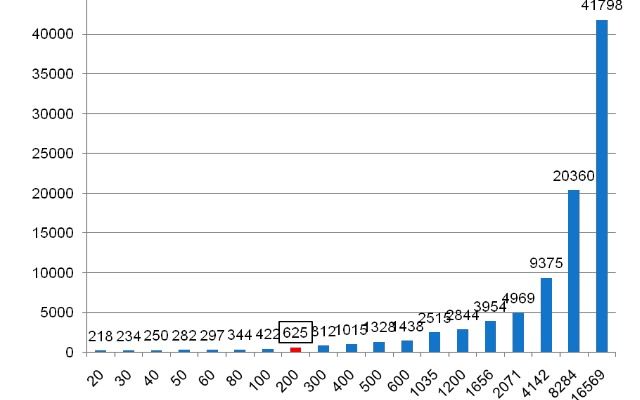
\includegraphics[width=1\textwidth]{images/runtimeSW.png}
    \caption[Runtime in ms of Gotoh for n/i ]{Runtime in ms of the local alignment, considering all base pairs n. If the mtDNA is chopped in 84 pieces of length 200, the calculation takes 625ms instead of 41,798 ms when considering the full length sequence}. 
    \label{fig:runtimeSW}    
\end{figure}
While this basic approach outperforms various tools in the runtime, it is still too slow to align large set of sequences with several thousand sequences. 

\subsection{K-mer Hash map based approach}
Given the high similarity of mtDNA sequences, the use of k-mer based approaches for identifying identical reads can skip the cost-expensive dynamic programming (either global or local alignment). Similar to BLAST \cite{Altschul1990}, a hashing scheme is used to match the exact k-mer, however without extending to maximal-length matches, but with the additional use of global alignment. The main idea is to use the hashing scheme to perform also the alignment while only 1 base is differing between the query and the reference sequence (as SNP or as indel) in an k-mer, and apply the global alignment as soon as 2 or more SNPs are differing on the short k-mers. The length of the k-mers needs to be longer than 16 bases, since one 15-mer exist, with exact matches on two different loci of the mtDNA reference rCRS.
%To use shorter k-mers, an optimization is presented in subsection \ref{align:optim}, to prevent hash collisions.
The presented approach requires a pre-calculation of the hash-table, which is not required if working solely with dynamic programming like in the $SW^{2}$ approach.
The hash table is implemented as a collision free hash map, since all keys are known when constructing the map. Therefore a perfect hash function gets applied, allowing for lookups of $\mathcal{O}(1)$ in all cases. While the key of the hash map is the hash value of the k-mer, the value is the starting position according the reference sequence rCRS. The calculation costs for building the hash-map for the rCRS with 20-mers is $\sim$ 30 ms, and has to be taken into account.
The algorithm for querying can be drafted as follows:
\begin{itemize}
\item 1. split query sequence of length $m$ into a list of chunks $c$ of length $k$
\item 2. iterate over each chunk $c_i$ of $m$ for $i=0; i= m/k$ and generated hash of $c$ = $h(c_i)$
\subitem{ 2.a) if $h(c_i)$ is not a key in the hash map $H$, assign value (=position) to temp variable and checking if the position is as expected (multiple of k, plus considering offset). If yes, back to 2. by taking the next hash $c_{i+1}(h)$ if position only differs by 1, insertion of 1 and set offset++, else perform Needleman-Wunsh, and count offsets if any }
\subitem 2.b) else if $h(c_i) \notin H$, find anchor $a$, by creating new hash by shifting    $h(c_i)+j for j =0; j<=k$ such that a match can be found. If $a$ as match in $H$ is found, perform NeedleMan Wunsh on all non-matching part, prior position of $a$. Continue with 2 for $h(c_i)+j$
\item correct according rules 1-3: 
\subitem  Rule 1 - Least number of Differences
\subitem Rule 2 - Maintain the AC repeat motif around position 523A-524C.
\subitem Rule 3 - Direction of indels in homopolymeric stretches is  to put  3’ (from right) instead of 5’ (from left). 
\end{itemize}
%There do exist further exceptions that need to be considered in 2.b)  
%\subsection{Optimizations: multi-map}\label{align:optim}
\section{Comparison to Data Structures}
Based on the GenBank data downloaded as variants as of October 2015\footnote{\url{http://www.ianlogan.co.uk/checker/genbank.htm}},  30.561 samples are considered for the evaluation. First the classification of the downloaded profiles to haplogroups is performed and in a second step, the fasta sequence files are written (total file size 506.8 MB). While the fasta sequence is alway unambiguous, the alignment is not always. To guarantee that the sequences used in HaploGrep 2 can be assigned the correct haplogroup, we downloaded all sequences from Genbank to take all sequences used for comparison with alternative software solutions.

By using parametrized test cases with JUnit\footnote{\url{http://www.junit.org/}} in the Eclipse software development environment\footnote{\url{www.eclipse.org/}} the comparison of aligned sequences to the variant files is performed for the haplogroup defining profiles from Phylotree. In a first test the gap penalties of the dynamic programming is set, so that the selected alignment with the least number of differences between the sample and the rCRS sequence is established. This corresponds to Rule 1 – Least number of Differences defined by Wilson \cite{Wilson2002}. Rule 2 defines the priorities in case of ambiguous alignments: insertions and deletions (indels) are to be prioritized over transition and transition over transversions. Further indels need to be considered from right to left instead of left to right. A rule shifting such position to the rightmost occurrence of the same base, e.g. Swith Waterman detects a deletion on T15940d, however the bases in the rCRS from 15940 to 15944 are all thymine, therefore the correct position is T15944d. 
\begin{table}[H]
\centering
\caption{k-mer hash based approach in HaploGrep 2}
\label{time:HG2}
\begin{tabular}{|l|l|l|}
\hline
Samples &  HaploGrep 2 &  Global alignments performed   \\ \hline
1,000    & 0.994 sec  &   908        \\ \hline
2,000    & 1.366 sec &   1,725        \\ \hline
5,000    & 2.284 sec &   3,710        \\ \hline
10,000   & 4.285 sec &   7,622        \\ \hline 
30,651   & 11.095 sec&  21,950    \\ \hline
\end{tabular}
\end{table}
\subsection{Suffix Trees}
As an implementation of a suffix tree, MUMmer is applied on the previously described data sets. MUMmer was used in version 3.23. Since MUMmers outputs a so called delta encoded file\footnote{\url{http://nebc.nerc.ac.uk/bioinformatics/documentation/mummer/nucmer.README}}, further processing with the show-snp program is required. Only after processing this snp file, it can be directly imported into HaploGrep, based on a Java based converter, written for the evaluation of the produced variants. Table \ref{tableMummer} reports the run time for the mtDNA sequences from GenBank as previously described, where \texttt{COMPLETETIME} is the time estimated by MUMmer, real time the console run time and the column \texttt{show-snp} represents the runtime to convert the delta encoded style to the resulting SNP file.  
\begin{table}[H]
\centering
\caption{MUMmer 3.23 Runtime: parameter -c 100 applied }
\label{tableMummer}
\begin{tabular}{|l|l|l|l|}
\hline
Samples &  Real Time &  \texttt{COMPLETETIME}  & \texttt{show-snp} \\ \hline
1,000    & 2.814 sec  &   2.25 sec  &  0.423 sec  \\ \hline
2,000    & 5.525s sec &   4.54 sec  &   0.757 sec \\ \hline
5,000    & 13.525s sec &   11.14 sec &  1.851 sec \\ \hline
10,000   & 27.240 sec  &   22.55 sec  &  3.701 sec\\ \hline 
30,651   & 82.483 sec  &  68.70 sec  & 11.140 sec\\ \hline
\end{tabular}
\end{table}
\subsection{FM-Index}
As previously described, an FM-Index efficiently handles the reference genome, and allows the search for maximum unique matches, as applied in the suffix tree, previously described. In this validation, the BWA MEM algorithm was applied, which works by extending alignments with maximal exact matches (therefore MEMs) and then extending seeds with the affine-gap Smith-Waterman algorithm (SW).    
BWA first needs to construct the FM-index for the reference, which is almost negligible for the rCRS reference sequence with 0.028 seconds real time (BWA version 0.7.12-r1039). 
\begin{table}[H]
\centering
\caption{BWA runtime}
\label{time:BWA:SMALT}
\begin{tabular}{|l|l|l|l|}
\hline
Samples &  \texttt{bwa mem}  &  \texttt{smalt k=20, s=20} &  \texttt{smalt k=13, s=13} \\ \hline
1,000    & 24.462   &    3m37.20sec &  6m29.977s\\ \hline
2,000    & 48.408   &    7m53.428sec &  13m7.032s\\ \hline
5,000    & 121.222  &   20m44.275s
  &  30m24.149s \\ \hline
10,000   & 239.089  &  40m26.542s   & 62m8.970s\\ \hline 
\end{tabular}
\end{table}

\subsection{Performance of mtDNA specific aligners}
Besides MUMmer, as an implementation of a suffix tree, and BWA operating on an FM-Index, the related methods MitoTool, mtDNAprofiler and Phy-mer are compared against the here presented hash-map based approach, included in HaploGrep 2, based on the datasets from GenBanks full mtDNA sequences.
\begin{table}[H]
\centering
\caption{Comparison mtDNA specific aligner}
\label{align:comp}
\begin{tabular}{|l|l|l|l|l|}
\hline
Run Time for & phy-mer &  MitoTool & mtDNAprofiler & HaploGrep2 \\ \hline
50 Samples  &  1690 sec  &    \begin{tabular}{@{}c@{}}1260 sec$^{1}$ \\ 105.55 sec$^{2}$\end{tabular}   &  110 sec$^{3}$ &  0.44 sec     \\ \hline

\end{tabular}
\end{table}
The resulting haplogroups are listed in the appendix Table \ref{app:table}, whereby the result of mtDNAprofiler was processed with HaploGrep 2 and yields the same haplogroup results and is therefore not reported separately. Further, as additional performance test, mappers/aligner for third-generation sequencing are compared: BWA MEM ONT2D, GraphMap, and Last.
\begin{table}[H]
\centering

\subsection{Optimizations: multi-threads}

\begin{table}[H]
\centering
\caption{k-mer hash based approach in HaploGrep 2}
\label{time:threads}
\begin{tabular}{|l|l|l|}
\hline
Samples &  HaploGrep 2 &  MUMmer 4.0.0beta   \\ \hline
1,000    & 0.417 sec  &   0.416        \\ \hline
2,000    & 0.790 sec &   0.768        \\ \hline
5,000    & 1.703 sec &   1.774        \\ \hline
10,000   & 4.285 sec &   3,365        \\ \hline 
\end{tabular}
\end{table}

\caption{Comparison Third-Generation Mapper}
\label{align:comp3Gen}
\begin{tabular}{|l|l|l|l|}
\hline
Run Time & BWA ONT2D & GraphMap & Last \\ \hline
1,000 &    22.185   &  23.012 (91.45 CPU time)  &    29.028     \\ \hline
2,000 &    42.773  &  46.120 (183.56 CPU time)   &   57.728    \\ \hline
5,000  &   105.294  &   114.437 (455.62 CPU time) &  142.383    \\ \hline
10,000 &   214.854  &  229.013 (911.88 CPU time) &  277.963      \\ \hline

\end{tabular}
\end{table}


\section{Conclusion and Outlook}
Several well established approaches to align nucleotide sequences with numerous algorithms facing this problem[blast(ncbi blast, psi-blast), fasta(fasta, ssearch, fastm, ggsearch), Hidden Markov Models (hmmer, sam) ] do exist. However only a few sequence alignment tools for mitochondrial DNA do exist, performing either poor regarding calculation time or nonsatisfying in the context of reliable alignment due to the special characteristics of mtDNA structure. Although there are several guidelines on how to align mtDNA data [Wilson Rules, SWGDAM-rules], expertise knowledge is still needed. We therefore designed a new sequence alignment tool for the fast and reliable alignment of full mitochondrial DNA sequence data. As a result we extend our mitochondrial workbench HaploGrep 2 with the herein described alignment module to allow an accurate and easy handling of mtDNA fasta files.
%De-novo vs. mapping assembly Wikipedia Artikel!! 
%Paper: A Practical Comparison of De Novo Genome Assembly Software Tools for Next-Generation Sequencing Technologies




